\documentclass[aspectratio=169,12pt]{beamer}

% ---------- packages ----------
\usepackage[T1]{fontenc}
\usepackage[utf8]{inputenc}
\usepackage{amsmath}
\usepackage{amsfonts}
\usepackage{amssymb}
%\usepackage{helvet}
%\renewcommand{\familydefault}{\sfdefault}
\usepackage{microtype}
\usepackage{newpxtext}
\usepackage{booktabs}
\usepackage{tikz}
\usetikzlibrary{arrows.meta,positioning,calc}
\usepackage{qrcode}
\usepackage{graphicx}
\graphicspath{{figures/}}
\usefonttheme{professionalfonts}
\usepackage{mathpazo}

% ---------- EDIT THESE ----------
\newcommand{\appurl}{https://YOUR-APP-NAME.streamlit.app}   % your deployed Streamlit link
\newcommand{\presenter}{Sovannvatanak PHAUT}
% --------------------------------

% ---------- colours (match the Streamlit app) ----------
\definecolor{ink}{HTML}{16313A}
\definecolor{teal}{HTML}{1F6F78}
\definecolor{tealtint}{HTML}{E3EEEE}
\definecolor{muted}{HTML}{9DB8BB}
\definecolor{fast}{HTML}{2E8B6A}
\definecolor{mid}{HTML}{B27A00}
\definecolor{slow}{HTML}{C0392B}
\definecolor{grey}{HTML}{4B6670}

\hypersetup{colorlinks=false,pdfborder={0 0 0}}
\setbeamertemplate{navigation symbols}{}
\setbeamercolor{background canvas}{bg=white}
\setbeamercolor{normal text}{fg=ink}
\setbeamercolor{structure}{fg=teal}
\setbeamercolor{item}{fg=teal}
\setbeamercolor{button}{bg=teal,fg=white}
\setbeamerfont{itemize/enumerate body}{size=\normalsize}
\setbeamertemplate{itemize items}[circle]
\setbeamertemplate{itemize item}{\color{teal}\textbullet}
\setbeamertemplate{itemize subitem}{\color{teal}--}

% ---------- clickable section tabs in the headline ----------
\newcommand{\navtab}[3]{% #1 = section number, #2 = target frame label, #3 = text
  \ifnum\insertsectionnumber=#1\relax
    \colorbox{teal}{\color{white}\strut\,#3\,}%
  \else
    \hyperlink{#2}{\colorbox{tealtint}{\color{ink}\strut\,#3\,}}%
  \fi\hspace{0.35em}}

\setbeamertemplate{headline}{%
  \leavevmode\hbox to\paperwidth{\hspace{0.9cm}\vbox to 1.0cm{\vfil
    \hbox{\footnotesize
      \navtab{1}{s-problem}{Problem}%
      \navtab{2}{s-data}{Data}%
      \navtab{3}{s-model}{Model}%
      \navtab{4}{s-results}{Results}%
      \navtab{5}{s-demo}{Live Demo}%
      \navtab{6}{s-wrap}{Wrap-up}}%
  \vfil}\hfil}}

\setbeamertemplate{footline}{%
  \leavevmode\hbox to\paperwidth{\hspace{0.9cm}\vbox to 0.8cm{\vfil
    \hbox to \dimexpr\paperwidth-1.8cm\relax{\scriptsize\color{grey}
      Delivery Time Prediction \textbullet\ AUPP Data Science Club\hfill\insertframenumber}\vfil}}}

\setbeamertemplate{frametitle}{%
  \vskip-0.15cm
  \hspace{0.1cm}{\Large\bfseries\color{ink}\insertframetitle}\par
  \vskip0.12cm
  {\color{teal}\hrule height 2pt}
  \vskip0.2cm}

\setbeamersize{text margin left=0.9cm,text margin right=0.9cm}

% little helpers
\newcommand{\bignum}[2]{{\bfseries\fontsize{30}{32}\selectfont\color{#1}#2}}
\newcommand{\card}[3]{% colour, number, caption
  \begin{tikzpicture}
    \node[draw=muted,fill=white,rounded corners=4pt,minimum width=3.3cm,minimum height=2.2cm,align=center,inner sep=6pt]
      {\bignum{#1}{#2}\\[2pt]{\small\color{grey}#3}};
  \end{tikzpicture}}

\title{How long will my food delivery take?}
\subtitle{Predicting delivery time with machine learning, and a live app}
\author{\presenter}
\institute{AUPP Data Science Club \textbullet\ Final Project}
\date{13 November 2026}

\begin{document}

% =============== TITLE ===============
\begin{frame}[plain,label=title]
  \vspace{0.5cm}
  \begin{tikzpicture}[remember picture,overlay]
    \fill[teal] (current page.south west) rectangle ([xshift=0.45cm]current page.north west);
  \end{tikzpicture}
  \hspace{0.6cm}\begin{minipage}{0.85\textwidth}\raggedright
    {\fontsize{30}{34}\selectfont\bfseries\color{ink}How long will my food\\delivery take?\par}
    \vspace{0.3cm}
    {\Large\color{teal}Predicting delivery time with machine learning, and a live app\par}
    \vspace{0.3cm}
    \begin{center}
    {\large\presenter\par}
    {\color{grey}AUPP Data Science Club, Final Project\par}
    {\color{grey}13 November 2026\par}
    {\color{grey}\LaTeX\par}
    \end{center}
    \vspace{0.1cm}
    \hyperlink{s-problem}{\beamergotobutton{Start}}
  \end{minipage}
\end{frame}

% =============== 1 PROBLEM ===============
\section{Problem}
\begin{frame}[label=s-problem]{Why predict delivery time?}
  \begin{columns}[T]
    \begin{column}{0.58\textwidth}
      \begin{itemize}
        \setlength\itemsep{0.55em}
        \item Customers want an \textbf{honest ETA}
        \item Restaurants and dispatchers need it to \textbf{plan couriers}
        \item \textbf{Goal:} predict delivery time in minutes from the order, the route and the courier
        \item A \textbf{regression} problem. Target: \texttt{Time\_taken (min)}
      \end{itemize}
    \end{column}
    \begin{column}{0.38\textwidth}
      
      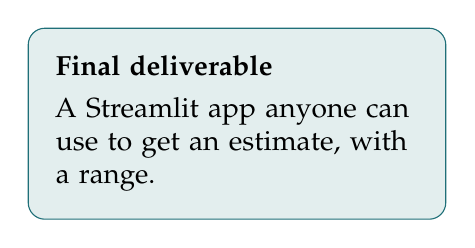
\begin{tikzpicture}
        \node[draw=teal,fill=tealtint,rounded corners=6pt,inner sep=10pt,text width=4.6cm,align=left]
          {\textbf{Final deliverable}\\[3pt]
           A Streamlit app anyone can use to get an estimate, with a range.};
      \end{tikzpicture}
    \end{column}
  \end{columns}
  \vfill
  \footnotesize\color{grey}Jump to:\ 
    \hyperlink{s-data}{\beamergotobutton{Data}}\ 
    \hyperlink{s-model}{\beamergotobutton{Model}}\ 
    \hyperlink{s-results}{\beamergotobutton{Results}}\ 
    \hyperlink{s-demo}{\beamergotobutton{Live demo}}
\end{frame}

% =============== 2 DATA ===============
\section{Data}
\begin{frame}[label=s-data]{The data: Zomato food delivery orders}
  \begin{itemize}
    \setlength\itemsep{0.45em}
    \item Kaggle: Zomato food delivery dataset. Each row is one order: route, weather, traffic, vehicle and courier
    \item Delivery times range from \textbf{10 to 54 minutes}
    \item The data comes from Indian cities
  \end{itemize}
  \vfill
  \centering
  %
  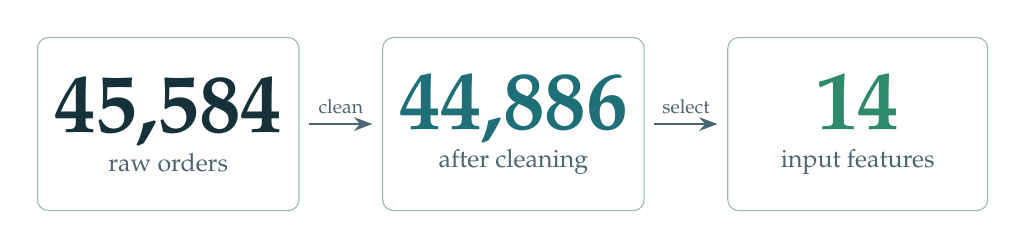
\begin{tikzpicture}[>=Stealth]
    \node (a) {\card{ink}{45,584}{raw orders}};
    \node[right=0.8cm of a] (b) {\card{teal}{44,886}{after cleaning}};
    \node[right=0.8cm of b] (c) {\card{fast}{14}{input features}};
    \draw[->,thick,color=grey] (a) -- node[above,font=\scriptsize]{clean} (b);
    \draw[->,thick,color=grey] (b) -- node[above,font=\scriptsize]{select} (c);
  \end{tikzpicture}
  \vfill
\end{frame}

\begin{frame}[label=s-clean]{Cleaning: what we fixed and why}
  \small\renewcommand{\arraystretch}{1.08}
  \begin{tabular}{@{}p{0.36\textwidth}p{0.6\textwidth}@{}}
    \toprule
    \textbf{Problem in the data} & \textbf{What we did}\\
    \midrule
    Padded text, \texttt{"NaN "} & Stripped spaces, made real blanks\\
    Mixed date and time formats & Auto-detected; built weekday, weekend, hour\\
    Only raw coordinates & Computed \textbf{distance in km}\\
    Codes that look like numbers & Kept as \textbf{categories}\\
    Pickup time & \textbf{Removed:} unknown at order time (leakage)\\
    Rows with 4+ blanks & Dropped (1.5\%); others filled in the pipeline\\
    \bottomrule
  \end{tabular}
\end{frame}

\begin{frame}[label=s-eda]{What the data shows}
  \centering
  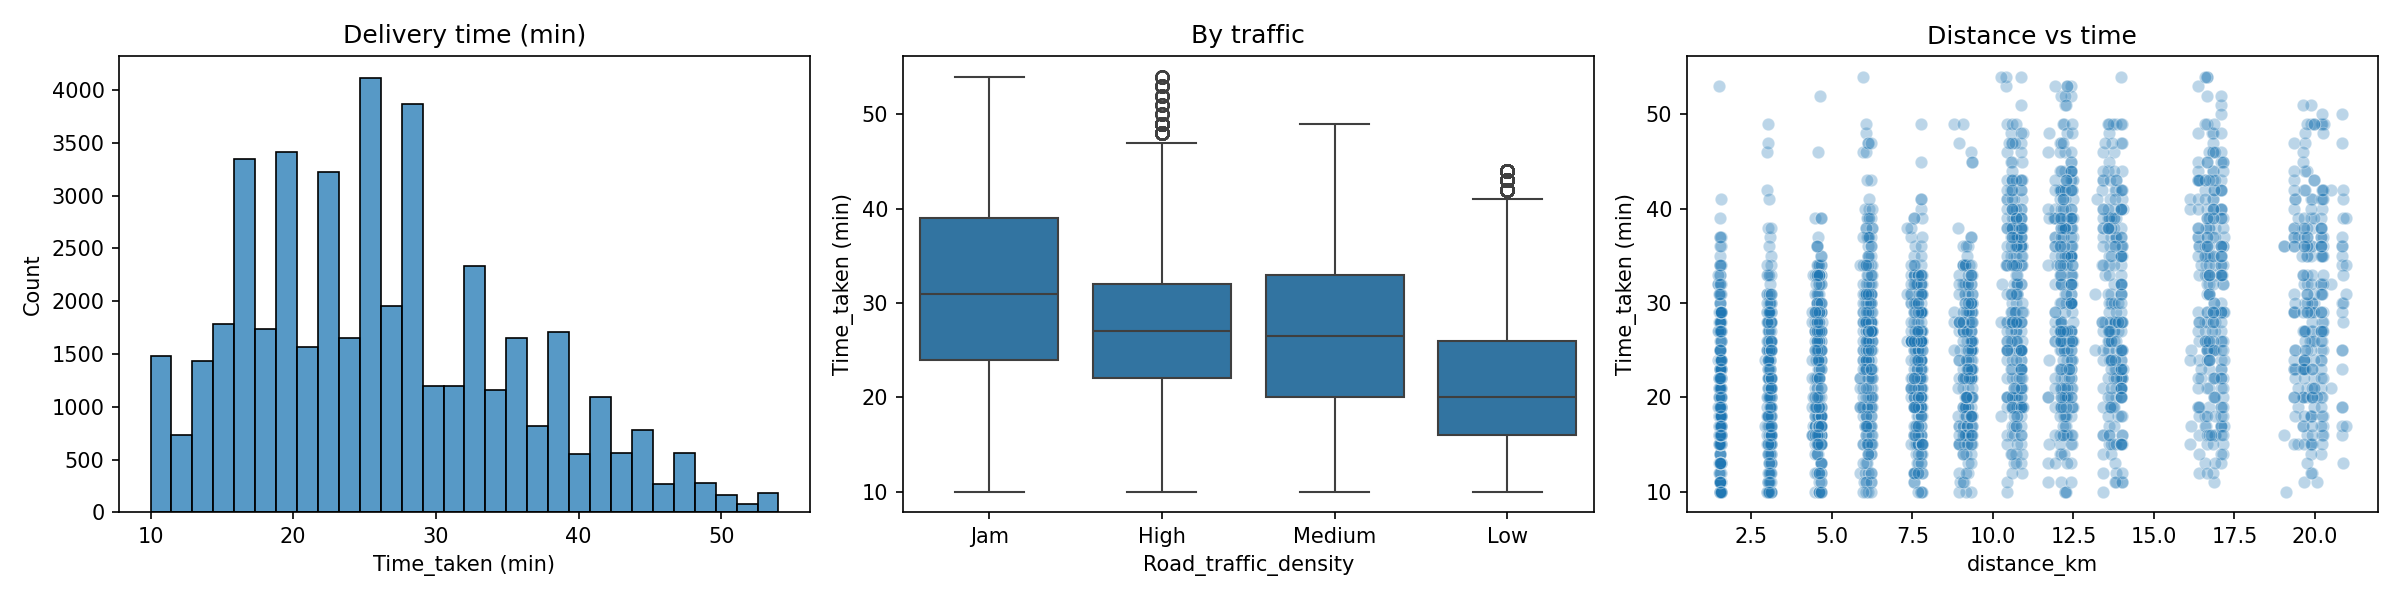
\includegraphics[width=0.97\textwidth]{eda_overview.png}\par
  \vspace{0.2cm}
  \begin{columns}[T]
    \begin{column}{0.32\textwidth}\small\textbf{Most orders take 15 to 30 min.} The longest are over 50.\end{column}
    \begin{column}{0.32\textwidth}\small\textbf{Traffic matters.} Median is about 31 min in a jam and about 20 min in light traffic.\end{column}
    \begin{column}{0.32\textwidth}\small\textbf{Distance alone is weak.} Times vary widely at every distance, so we need several features together.\end{column}
  \end{columns}
\end{frame}

% =============== 3 MODEL ===============
\section{Model}
\begin{frame}[label=s-model]{How the model was built}
  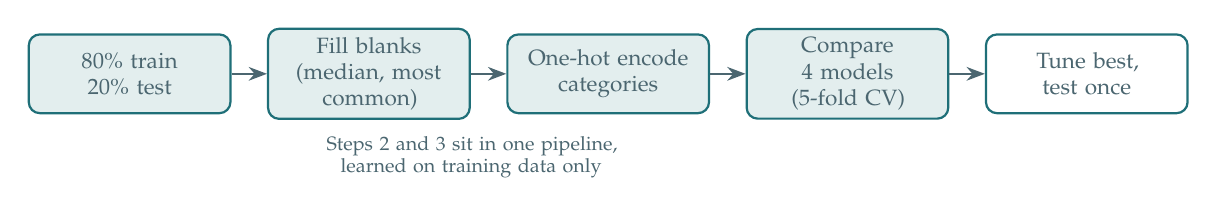
\begin{tikzpicture}[>=Stealth,
      stp/.style={draw=teal,fill=tealtint,rounded corners=4pt,minimum height=1.0cm,text width=2.35cm,align=center,font=\footnotesize,inner sep=3pt},
      every path/.style={thick,color=grey}]
    \node[stp] (s1) {80\% train\\20\% test};
    \node[stp,right=0.45cm of s1] (s2) {Fill blanks\\(median, most common)};
    \node[stp,right=0.45cm of s2] (s3) {One-hot encode\\categories};
    \node[stp,right=0.45cm of s3] (s4) {Compare 4 models\\(5-fold CV)};
    \node[stp,right=0.45cm of s4,fill=white] (s5) {Tune best,\\test once};
    \draw[->] (s1)--(s2); \draw[->] (s2)--(s3); \draw[->] (s3)--(s4); \draw[->] (s4)--(s5);
    \node[below=0.08cm of s2.south east,anchor=north,font=\scriptsize,color=grey,text width=6.4cm,align=center] {Steps 2 and 3 sit in one pipeline, learned on training data only};
  \end{tikzpicture}
  
  %
  {\small\textbf{Cross-validation error (average miss, minutes). Lower is better.}}\par\vspace{0.05cm}
  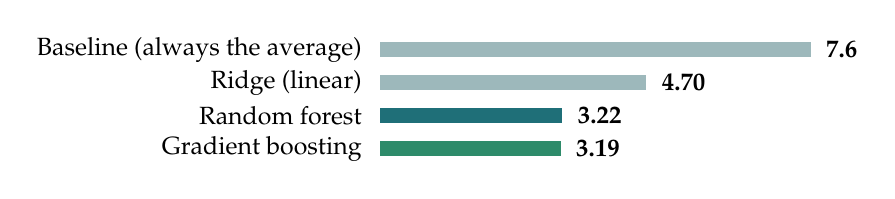
\begin{tikzpicture}[x=0.72cm,y=0.42cm]
    \foreach \name/\val/\col [count=\i] in {Baseline (always the average)/7.6/muted, Ridge (linear)/4.70/muted, Random forest/3.22/teal, Gradient boosting/3.19/fast}{
      \node[anchor=east,font=\small] at (-0.15,-\i) {\name};
      \fill[\col] (0,-\i-0.22) rectangle ({\val},-\i+0.22);
      \node[anchor=west,font=\small\bfseries] at ({\val+0.1},-\i) {\val};
    }
  \end{tikzpicture}\par
  \footnotesize\color{grey}The gap between Ridge and the tree models shows the relationships are not linear.
\end{frame}

% =============== 4 RESULTS ===============
\section{Results}
\begin{frame}[label=s-results]{Results on 8,978 orders the model never saw}
  \centering
  \normalsize\renewcommand{\arraystretch}{1.3}
  \begin{tabular}{@{}lrr@{}}
    \toprule
    & \textbf{Guess the average} & \textbf{Our model}\\
    \midrule
    Average error (MAE) & 7.59 min & \textbf{\color{fast}3.16 min}\\
    RMSE & 9.39 min & \textbf{\color{fast}3.97 min}\\
    $R^2$ & 0.00 & \textbf{\color{fast}0.82}\\
    Orders within $\pm5$ min & 38\% & \textbf{\color{fast}81\%}\\
    \bottomrule
  \end{tabular}\par
  \vspace{0.2cm}
  \normalsize Typically off by about \textbf{3 minutes}. Cross-validation error (3.15) matches the test error, so the model is \textbf{not overfit}.\par
  \vfill
  \footnotesize\hyperlink{s-errors}{\beamergotobutton{Where do the errors fall?}}
\end{frame}

\begin{frame}[label=s-errors]{Where the errors fall}
  \centering
  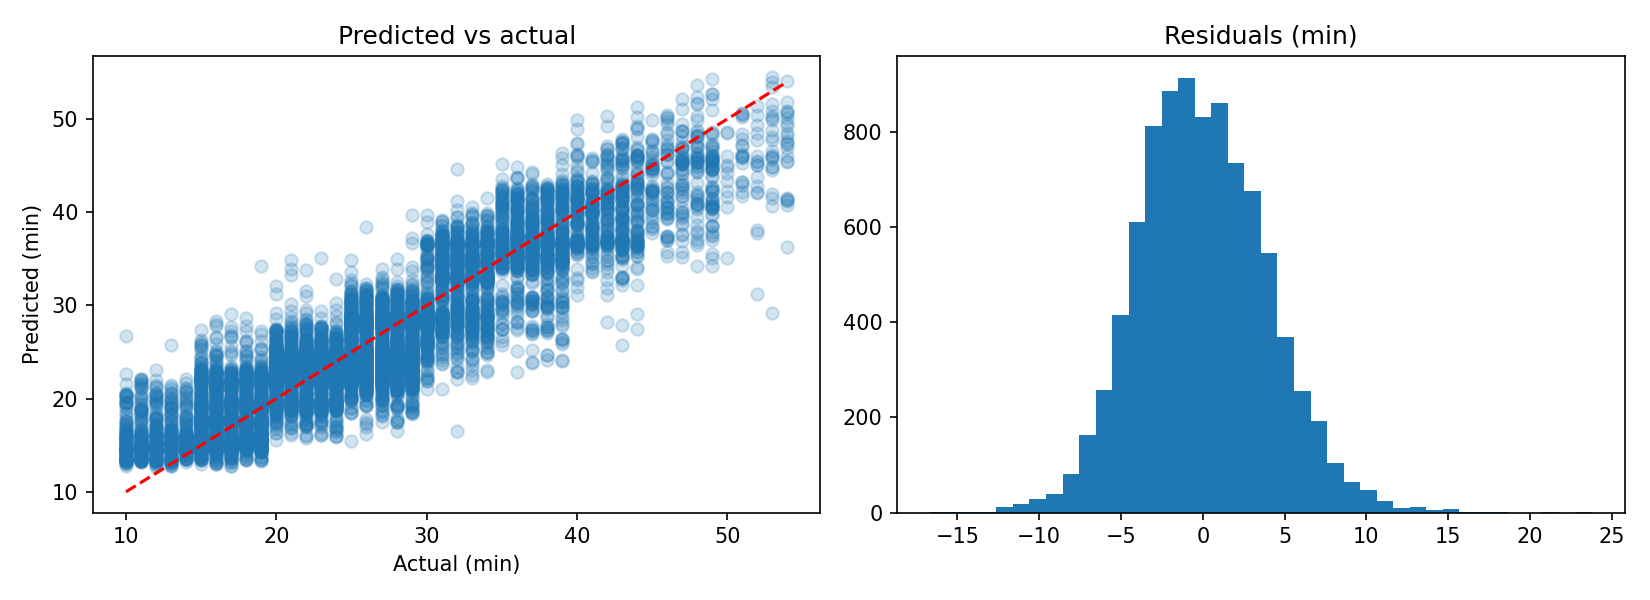
\includegraphics[width=0.78\textwidth]{model_eval.png}\par
  \vspace{0.15cm}
  {\small Left: predicted vs actual (red line = perfect). Right: errors are centred on 0 and mostly within $\pm$5 min.}\par
  \small\color{grey}Very fast and very slow orders are pulled toward the average.
\end{frame}

\begin{frame}[label=s-drivers]{What drives delivery time}
  \begin{columns}[c]
    \begin{column}{0.5\textwidth}
      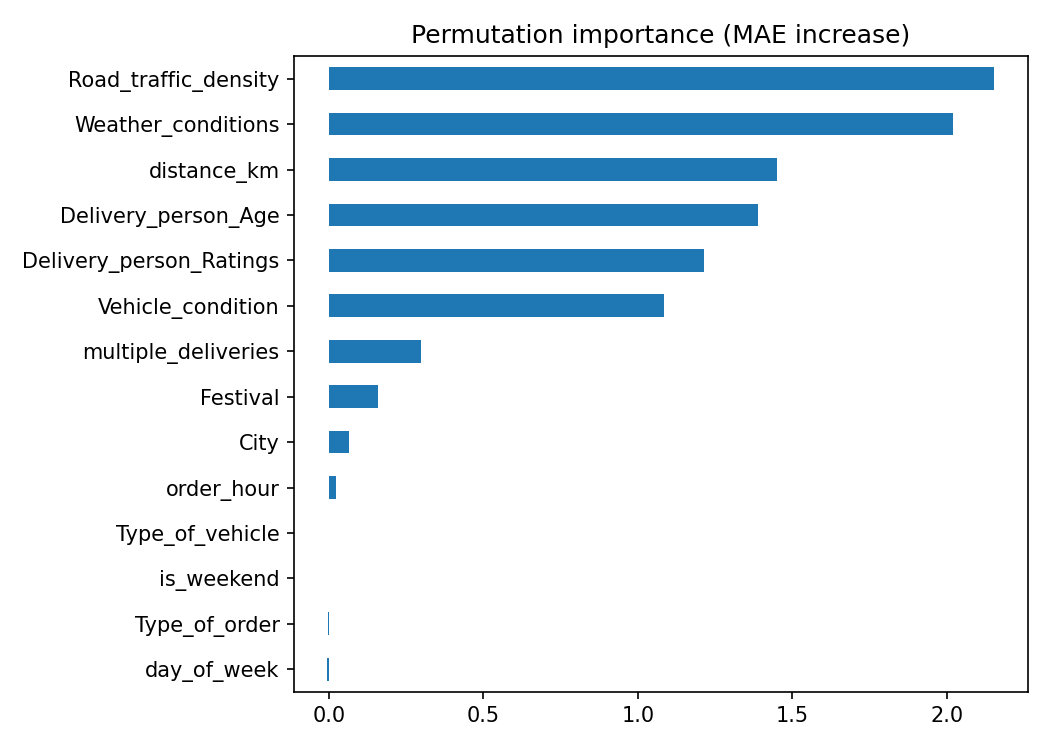
\includegraphics[width=\textwidth]{feature_importance.png}
    \end{column}
    \begin{column}{0.46\textwidth}
      \begin{itemize}
        \setlength\itemsep{0.5em}
        \item \textbf{Traffic} and \textbf{weather} matter most
        \item Then \textbf{distance}, courier \textbf{age}, \textbf{rating} and vehicle condition
        \item Weekday, hour and order type add almost nothing
      \end{itemize}
      \vspace{0.2cm}
      \scriptsize\color{grey}Importance = how much the error grows when one column is shuffled. It shows what the model uses, not what causes delays.
    \end{column}
  \end{columns}
\end{frame}

% =============== 5 DEMO ===============
\section{Live Demo}
\begin{frame}[label=s-demo]{Try it live}
  \begin{columns}[c]
    \begin{column}{0.4\textwidth}
      \centering
      \qrcode[height=3.6cm]{\appurl}\par
      \vspace{0.15cm}
      {\scriptsize\href{\appurl}{\color{teal}\underline{\appurl}}}
    \end{column}
    \begin{column}{0.56\textwidth}
      {\bfseries Three things to try}
      \begin{enumerate}
        \setlength\itemsep{0.55em}
        \item Press \textbf{Quiet sunny day}, then \textbf{Rush hour in a storm}, and watch the estimate move
        \item Open \textbf{What changes the time} to see one input at a time
        \item Save two orders and \textbf{compare} them side by side
      \end{enumerate}
      \vspace{0.2cm}
      \hyperlink{demo-backup}{\beamergotobutton{Backup screenshot}}
    \end{column}
  \end{columns}
\end{frame}

% =============== 6 WRAP-UP ===============
\section{Wrap-up}
\begin{frame}[label=s-wrap]{Takeaways and limits}
  \begin{columns}[T]
    \begin{column}{0.48\textwidth}
      {\bfseries\color{fast}What we learned}
      \begin{itemize}
        \setlength\itemsep{0.3em}
        \item Typical error \textbf{about 3 min}; \textbf{81\%} of orders within 5 min
        \item Traffic, weather, distance and the courier drive the time
        \item The model is packaged as a \textbf{live app}
      \end{itemize}
    \end{column}
    \begin{column}{0.48\textwidth}
      {\bfseries\color{slow}Limits and next steps}
      \begin{itemize}
        \setlength\itemsep{0.3em}
        \item Indian-city data: retrain on \textbf{local data} for Phnom Penh
        \item Random split, not tested over time
        \item Courier details are unknown to a customer, so it suits \textbf{dispatchers}
        \item Next: live traffic, time-based testing
      \end{itemize}
    \end{column}
  \end{columns}
\end{frame}

% =============== CLOSING ===============
\begin{frame}[label=s-thanks]{Thank you!}
  \vspace{0.6cm}
  \centering
  {\Large Try the app:\par}
  \vspace{0.3cm}
  {\large\href{\appurl}{\color{teal}\underline{\appurl}}\par}
\end{frame}

\appendix

\begin{frame}[label=demo-backup]{Backup: the app}
  \centering
  \IfFileExists{figures/app_screenshot.png}{%
    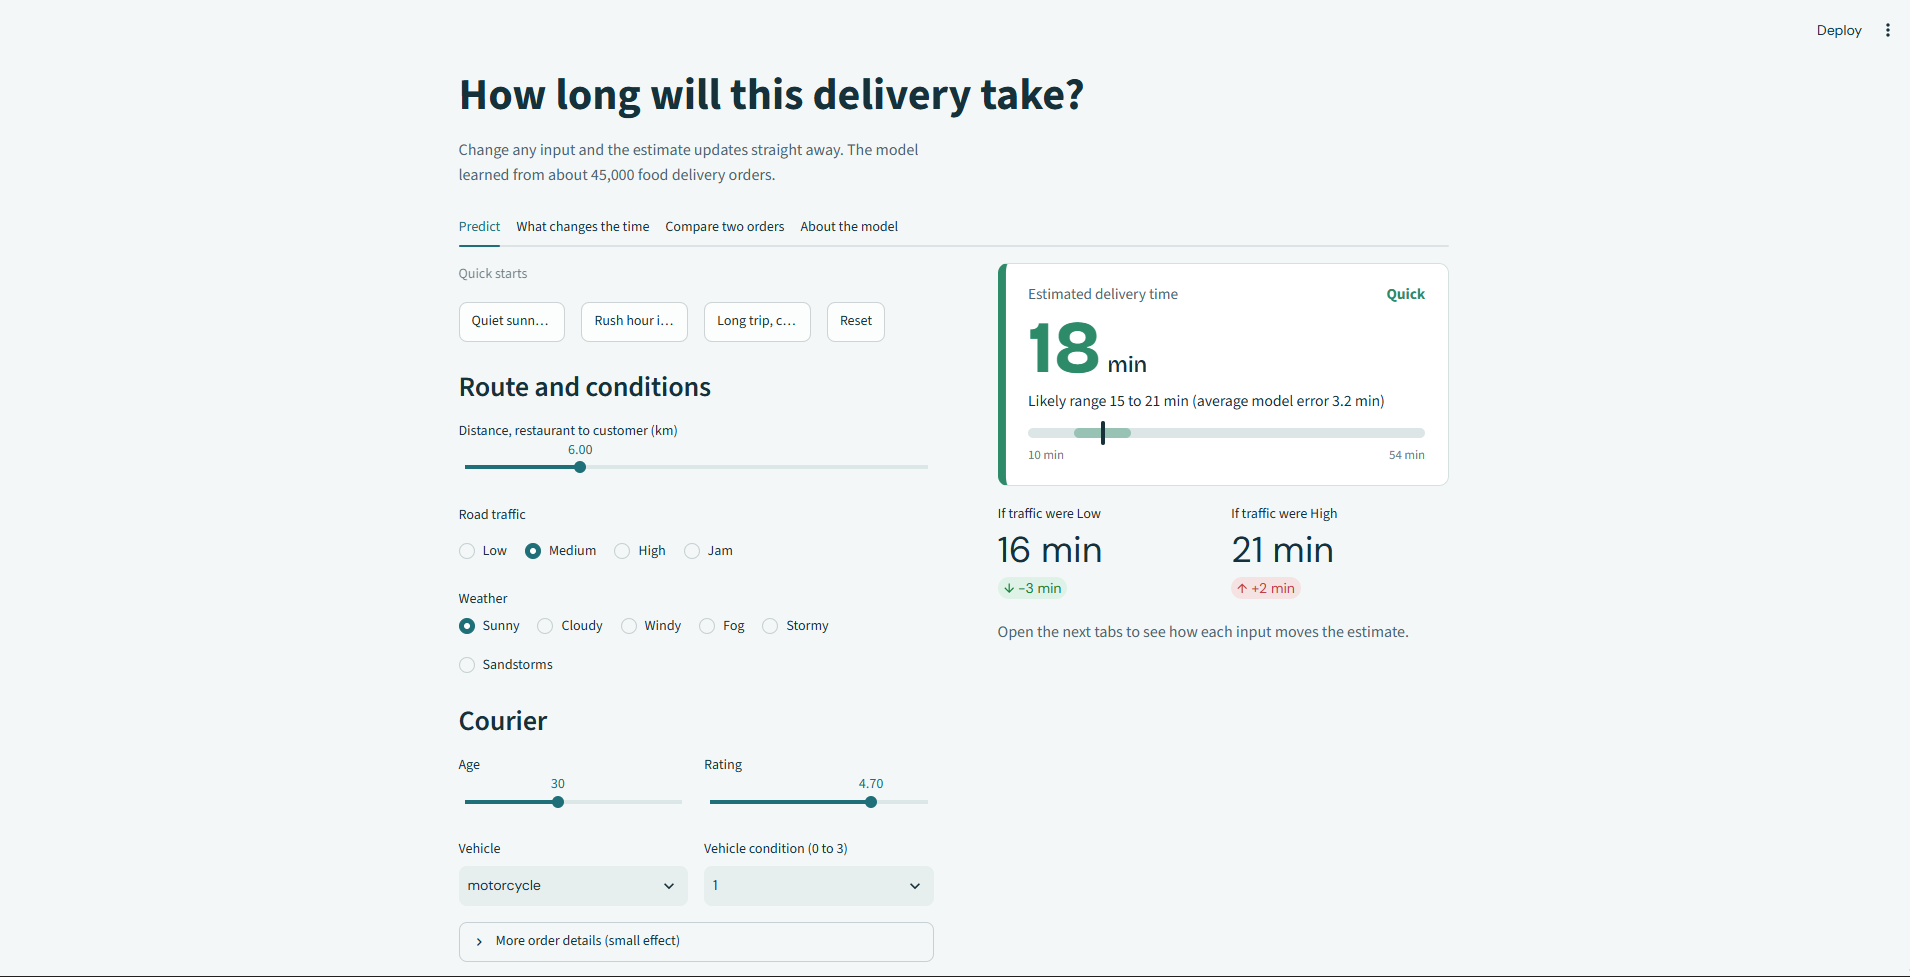
\includegraphics[height=0.72\textheight]{app_screenshot.png}}{%
    \fbox{\parbox{0.7\textwidth}{\centering\vspace{1cm}Save a screenshot of your app as\\\texttt{figures/app\_screenshot.png}\vspace{1cm}}}}
  \vfill
  \hyperlink{s-demo}{\beamerreturnbutton{Back to demo}}
\end{frame}

\end{document}